\section{genericFlatMc.h File Reference}
\label{genericFlatMc_8h}\index{genericFlatMc.h@{genericFlatMc.h}}
{\tt \#include \char`\"{}genericInterface.h\char`\"{}}\par
{\tt \#include \char`\"{}genericEvents.h\char`\"{}}\par
{\tt \#include \char`\"{}../../../util/genericData.h\char`\"{}}\par
{\tt \#include \char`\"{}../interfaces/processor.h\char`\"{}}\par
{\tt \#include \char`\"{}../../data\_\-types/impl/highLevelPacket.h\char`\"{}}\par
{\tt \#include \char`\"{}../../../memctrl/request.h\char`\"{}}\par
{\tt \#include $<$fstream$>$}\par
{\tt \#include $<$deque$>$}\par


Include dependency graph for genericFlatMc.h:\nopagebreak
\begin{figure}[H]
\begin{center}
\leavevmode
\includegraphics[width=420pt]{genericFlatMc_8h__incl}
\end{center}
\end{figure}


This graph shows which files directly or indirectly include this file:\nopagebreak
\begin{figure}[H]
\begin{center}
\leavevmode
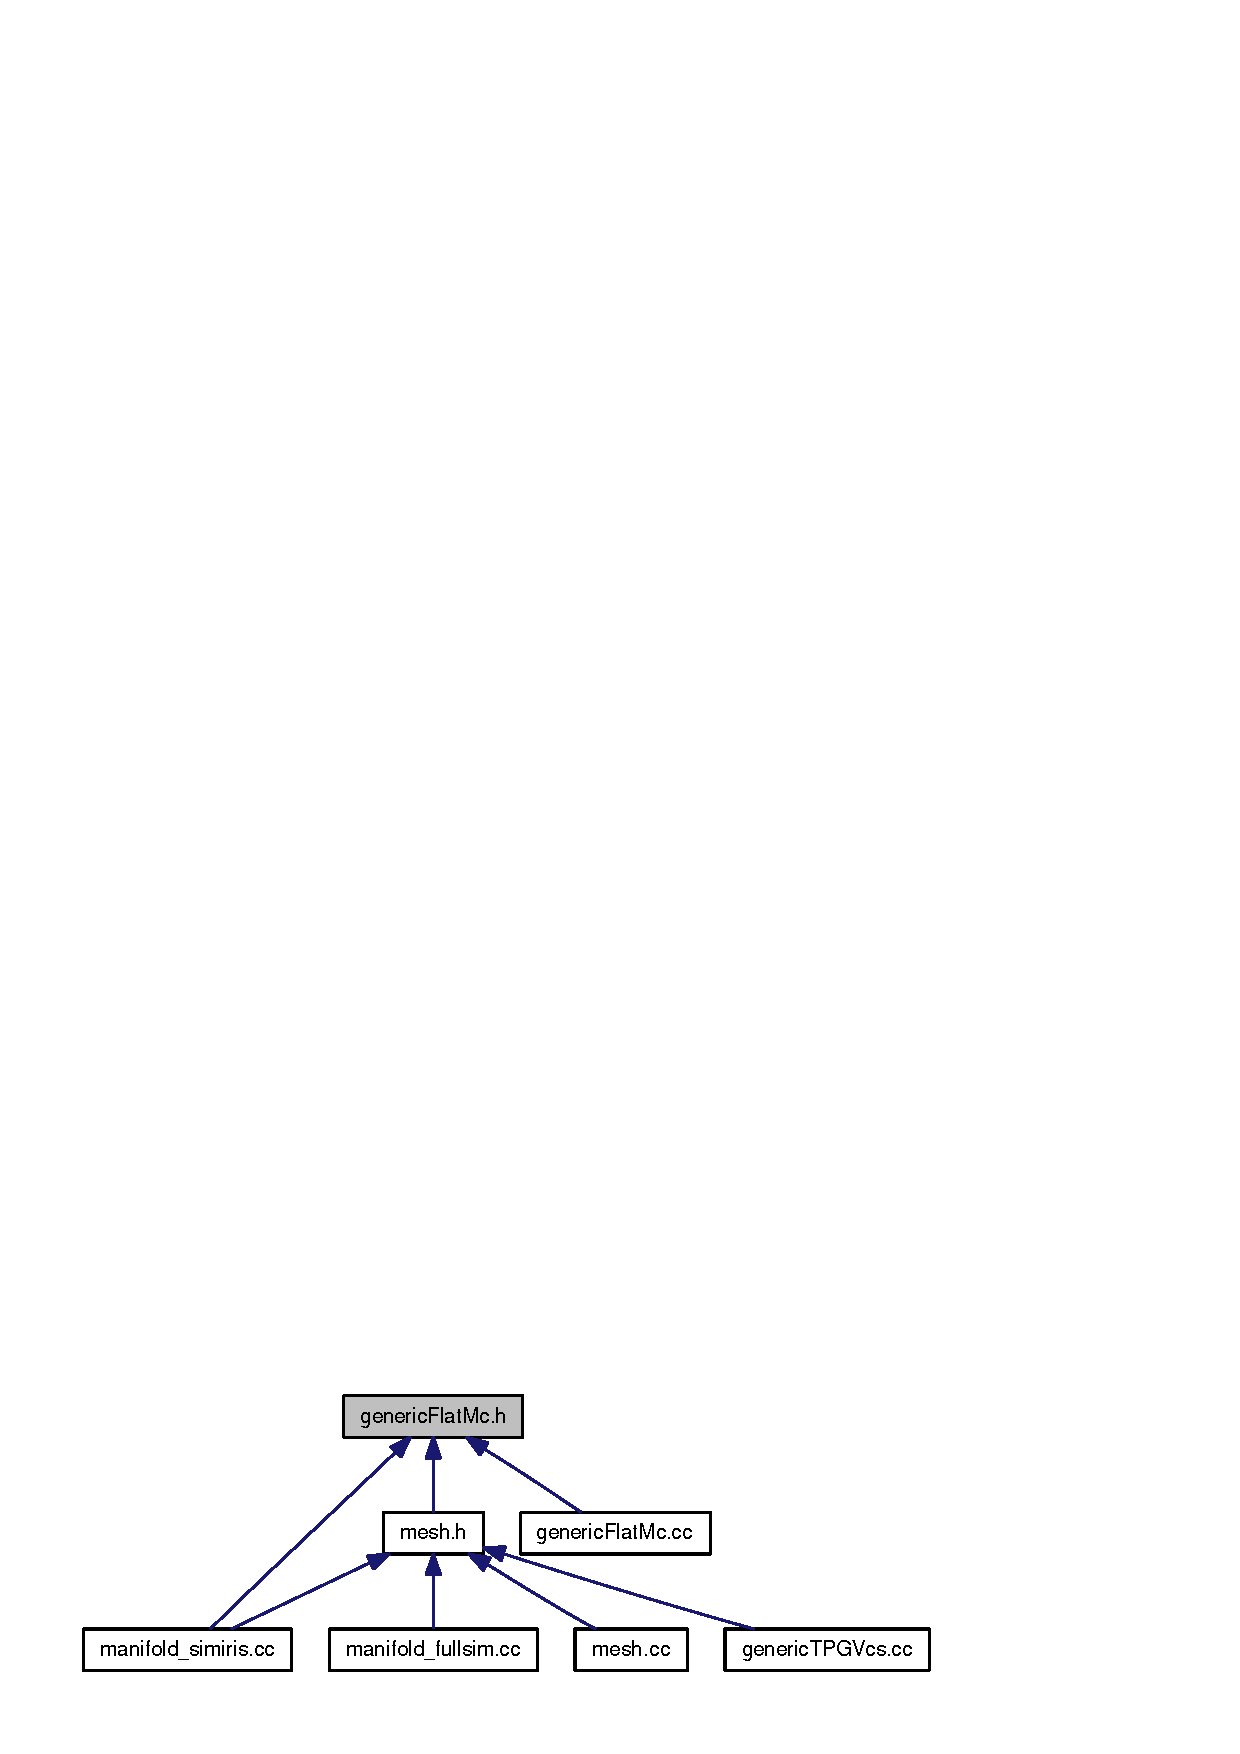
\includegraphics[width=225pt]{genericFlatMc_8h__dep__incl}
\end{center}
\end{figure}
\subsection*{Classes}
\begin{CompactItemize}
\item 
class {\bf GenericFlatMc}
\end{CompactItemize}
\subsection*{Defines}
\begin{CompactItemize}
\item 
\#define {\bf DEFAULT\_\-RAN\_\-MAX\_\-TIME}~100
\item 
\#define {\bf MAX\_\-ADDRESS}~3
\end{CompactItemize}


\subsection{Define Documentation}
\index{genericFlatMc.h@{genericFlatMc.h}!DEFAULT\_\-RAN\_\-MAX\_\-TIME@{DEFAULT\_\-RAN\_\-MAX\_\-TIME}}
\index{DEFAULT\_\-RAN\_\-MAX\_\-TIME@{DEFAULT\_\-RAN\_\-MAX\_\-TIME}!genericFlatMc.h@{genericFlatMc.h}}
\subsubsection[{DEFAULT\_\-RAN\_\-MAX\_\-TIME}]{\setlength{\rightskip}{0pt plus 5cm}\#define DEFAULT\_\-RAN\_\-MAX\_\-TIME~100}\label{genericFlatMc_8h_95a6218d50e244f6e58b6cca098c1d65}




Definition at line 14 of file genericFlatMc.h.\index{genericFlatMc.h@{genericFlatMc.h}!MAX\_\-ADDRESS@{MAX\_\-ADDRESS}}
\index{MAX\_\-ADDRESS@{MAX\_\-ADDRESS}!genericFlatMc.h@{genericFlatMc.h}}
\subsubsection[{MAX\_\-ADDRESS}]{\setlength{\rightskip}{0pt plus 5cm}\#define MAX\_\-ADDRESS~3}\label{genericFlatMc_8h_aba07841c3e227bc8bdd8ccdad149349}




Definition at line 15 of file genericFlatMc.h.

Referenced by GenericRPG::init\_\-generator().